\taskpic{Жонглер держит за концы невесомую, нерастяжимую нить, на 
которую нанизаны два шарика массой $m$ каждый, могущие без трения 
скользить по ней. Крайние участки нити всегда составляют угол 
$\alpha$ с вертикалью, а сила натяжения нити постоянна и равна $T$. За 
какое время шарики столкнутся, если в начальный момент они 
неподвижны и находятся на одной высоте на расстоянии $L$ друг от 
друга?}{
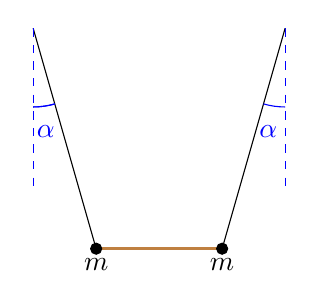
\begin{tikzpicture}[>=latex]
  \draw (0.4,3.6) -- (1.2,0.8);
  \draw (3.6,3.6) -- (2.8,0.8);
  \draw [dashed,blue] (0.4,3.6) -- +(0,-2);
  \draw [blue] (0.4,3.6) ++(0,-1) arc (-90:-90+atan(0.8/2.8):1);
  \draw [dashed,blue] (3.6,3.6) -- +(0,-2);
  \draw [blue] (0.4,3.6) ++(0,-1) arc (-90:-90+atan(0.8/2.8):1) node
  [below=10,right=-10] {$\alpha$};
  \draw [blue] (3.6,3.6) ++(0,-1) arc (-90:-90-atan(0.8/2.8):1) node
  [below=10,right=-5] {$\alpha$};

  \draw [very thick,brown] (1.2,0.8) -- (2.8,0.8);
  \filldraw [black] (1.2,0.8) circle (0.07) node[below] {$m$};
  \filldraw [black] (2.8,0.8) circle (0.07) node[below] {$m$};;
\end{tikzpicture}
}

\task{Мальчик раскручивает веревку длиной $L$ с привязанным к ее 
концу камнем. В момент, когда траектория камня представляет 
собой окружность в горизонтальной плоскости на высоте $h$ от 
земли, а угловая скорость вращения равна $\omega$, камень отрывается 
от веревки. Найти расстояние от точки на земле, где стоит мальчик, 
до точки падения камня. Сопротивлением воздуха пренебречь.}

\taskpic{На рисунке две прямые полосы облаков A и B (вид сверху), 
находящиеся на разных высотах. Векторы скорости ветра на этих 
высотах $\vec v_A$ и $\vec v_B$ также показаны на рисунке. Объясните, как 
построить вектор скорости движения по поверхности земли точки 
пересечения O теней облаков.}{
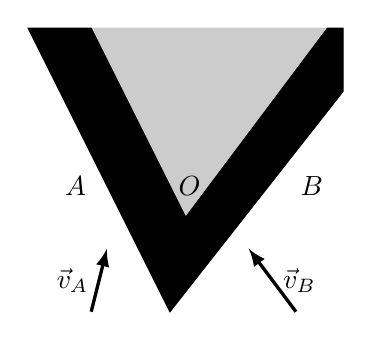
\begin{tikzpicture}[>=latex]
  \filldraw[black!20!white] (0.8,4) -- ++(1.2,-2.4) -- +(1.8,2.4) -- cycle;
  \filldraw[black] (0.8,4) -- (0,4) -- ++(1.5*1.2,1.5*-2.4) -- ++(2.2,2.8)
  -- ++(0,0.8) -- ++(-0.2,0) -- ++(-1.8,-2.4) -- cycle;
  \draw (0.6,2) node {$A$};
  \draw (3.6,2) node {$B$};
  \draw (2.05,2) node {$O$};
  \draw[very thick,->] (0.8,0.4) -- ++(0.2,0.8) node[midway, left]
  {$\vec{v}_A$};
  \draw[very thick,->] (3.4,0.4) -- ++(-0.6,0.8) node[midway, right]
  {$\vec{v}_B$};
\end{tikzpicture}
}

\task{По прямому участку железнодорожного пути движется вагон с 
ускорением 2{,}8~м/с$^2$. В вагоне мальчик пускает игрушечный состав 
по рельсам, расположенным поперек вагона. Ускорение состава 
относительно пола вагона равно 2,1~м/с$^2$. Найти абсолютную 
величину ускорения игрушечного состава относительно земли.}

\taskpic{Две одинаковые очень массивные шайбы, радиуса $R$ каждая, 
двигаются по скользкой горизонтальной плоскости навстречу друг 
другу со скоростями $v$ по одной прямой. Между ними, на равном 
расстоянии от них,  лежит шайба очень маленькой массы, радиуса  $r$. 
 Ее центр находится на расстоянии $d$ от прямой, соединяющей 
центры тяжелых шайб. Какую скорость приобретет легкая шайба 
после того, как шайбы разлетятся? Все шайбы жесткие 
(недеформируемые).}{
\begin{tikzpicture}[>=latex]
   \node[circle,draw,minimum size=20,very thick,fill=gray] at (0.5,2) (a) {};
   \node[circle,draw,minimum size=20,very thick,fill=gray] at (3.5,2) (b) {};
   \draw[dashed,thick] (a.east) -- (b.west);
   \draw[->,very thick] (a.east) -- ++(0.4,0) node [above] {$v$};
   \draw[->,very thick] (b.west) -- ($(b.west) + (-0.4,0)$) node [above] {$v$};
   \filldraw[red] ($(a.east)!0.5!(b.west)$) ++ (0,-0.3) circle (0.1);
   \draw[blue!80,dashed,dash pattern=on 1 pt off 1pt]
   ($(a.east)!0.5!(b.west)$) -- ++(0,-0.3);
   \draw[->,blue!80] (1,1) node[left] {$d$} to[out=0,in=180] (1.9,1.85);
\end{tikzpicture}
}

\taskpic{В точках A и B жесткого невесомого стержня укреплены два 
маленьких шарика. В точке O стержень закреплен и может свободно 
вращаться в вертикальной плоскости. В начальный момент времени 
стержень отклоняют от вертикального положения на очень 
маленький угол и отпускают. Найти силу, действующую на шарик В со 
стороны стержня в момент, когда угол между стержнем и вертикалью 
равен $\alpha$. Масса каждого груза $m$, длина стержня $L$, 
OA=AB.}{
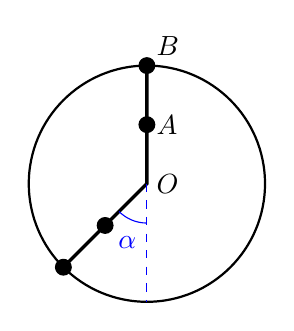
\begin{tikzpicture}[>=latex]
  \draw[thick] (2,2) circle (1.5);
  \draw[very thick] (2,3.5) -- (2,2) -- ++(-135:1.5);
  \filldraw[black] (2,2.75) circle (0.1) node[right] {$A$};
  \filldraw[black] (2,3.5) circle (0.1) node[above right] {$B$};
  \draw (2,2) node[right] {$O$};
  \filldraw[black] (2,2) ++(-135:0.75) circle (0.1);
  \filldraw[black] (2,2) ++(-135:1.5) circle (0.1);

  \draw[dashed,blue] (2,2) -- ++(0,-1.5);
  \draw[blue] (2,2) ++ (0,-0.5) arc (-90:-135:0.5);
  \draw[blue] (1.75,1.25) node {$\alpha$};
\end{tikzpicture}
}

\taskpic{Массивная бусинка нанизана на невесомую нерастяжимую нить 
длиной $L$, по которой может скользить без трения. Концы нити 
прикреплены к невесомым кольцам, которые могут свободно 
скользить по горизонтальному и вертикальному стержням. В 
начальный момент бусинку удерживают в таком положении, чтобы 
нить и стержни составляли квадрат. Бусинку отпускают. Найдите ее 
ускорение сразу после этого и время, за которое она достигнет 
вертикального стержня.}{
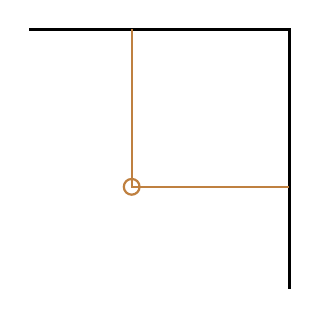
\begin{tikzpicture}[>=latex]
   \draw[very thick] (0.2,3.5) -- ++(3.3,0) -- ++(0,-3.3);
   \draw[thick,brown] (1.5,3.5) -- ++(0,-2) -- ++(2,0);
   \draw[thick,brown] (1.5,1.5) circle (0.1);
\end{tikzpicture}
}

\task{В чайнике нагревают воду кипятильником, подключенным к 
источнику постоянного напряжения $U$. Масса воды $m$, а ее удельная 
теплоемкость $c$. Начальная температура $T_0$. Через какое время 
вода закипит? Всеми потерями тепла и неоднородностью нагревания 
воды пренебречь. Электрическое сопротивление кипятильника 
зависит от температуры линейно: $R = R_0 + \alpha T$, где $\alpha$ и $R_0$ --- 
постоянные величины.}

\task{Наклонная плоскость имеет угол с горизонталью $\alpha$. По ней 
запускают косо вверх под углом $\beta$ к горизонтали две 
цилиндрические шайбы, массой $m$ каждая, лежащие точно одна на 
другой (по центру). Коэффициент трения между шайбами $\mu$, а между 
нижней шайбой и плоскостью $\mu_0$. Какова сила, с которой действует 
верхняя шайба на нижнюю  в верхней точке их траектории, если $\mu$ 
достаточно, чтобы шайбы не проскальзывали друг по другу? Может ли 
начаться такое проскальзывание, если его нет сначала? Какие еще 
начальные данные нужны для ответа на эти вопросы? }

\taskpic{Тело находится на абсолютно гладкой наклонной плоскости с 
углом $\alpha$ у основания. С помощью невесомых нерастяжимых нитей, 
перекинутых через блоки, находящиеся в основании и вершине 
наклонной плоскости, к телу привязан груз, имеющий массу $M$. Нити, 
подходящие к грузу, составляют с вертикалью и горизонталью углы 
$\beta$. Вся система находится в состоянии покоя.
Определите силы натяжения нитей и массу тела, трением в блоках 
пренебречь.
Проанализируйте, как изменятся ответы, если принять, что между 
телом и наклонной плоскостью существует трение (коэффициент 
трения $\mu$).}{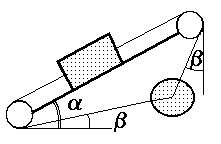
\includegraphics[width=3cm]{d10_10.png}}

\task{Велосипедист ускоряется так, что $av=C$, где $v$ --- скорость 
велосипедиста, $a$ --- ускорение, а $C$ --- некоторая постоянная 
величина. Найдите время, за которое его скорость увеличится от 
$v_1$ до $v_2$.}

\taskpic{На горизонтальном столе находится тело с массой $M_1=2\mbox{ кг}$. 
Коэффициент трения скольжения тела о поверхность $\mu=0{,}05$. К телу 
с помощью нити, перекинутой через блок, привязано вертикально 
висящее тело с массой $M_2$.
Постройте графики зависимости:
\begin{itemize}
\item силы трения от $M_2$;
\item ускорения тел от $M_2$;
\item силы натяжения нити от $M_2$.
\end{itemize}}{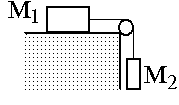
\includegraphics[width=3cm]{d10_12.png}}

\taskpic{В воде плавает однородный прямоугольный параллелепипед 
массой $M$. На середине одного из его ребер сидит воробей, так что 
противоположное ребро расположено в плоскости поверхности воды. 
Определите массу воробья $m$, если известно, что угол наклона 
параллелепипеда мал. Известно, что центр тяжести треугольника 
лежит на 1/3 его медианы.}{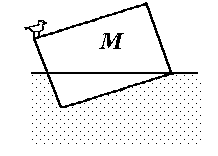
\includegraphics[width=3cm]{d10_13.png}}

\taskpic{Однородный проводящий контакт изогнут в виде дуги угла 
$2\pi-\alpha$. Вокруг центра дуги вращается с очень большой скоростью 
проводящий отрезок сопротивления $R$, так что контакт между 
отрезком и дугой идеальный. Сопротивление дуги равно 
сопротивлению отрезка. Устройство подключено к батарейке с 
постоянным напряжением $U$. Определить заряд, протекший по цепи за 
время $t$, и выделившееся тепло за это время. Сопротивлением 
подводящих проводов пренебречь.}{
\begin{tikzpicture}
  \draw[thick] (2,3) arc (45:315:1);
  \coordinate (a) at ($ (2,3)!1cm!(1.5,2.5) $);
  \coordinate (b) at ($ (a)!1cm!-90:(2,3)$);
  \draw[dashed,blue] (2,3) -- (a) -- ++(-45:1);
  \draw[fill=black] (a) circle (0.05);
  \draw[|-|] (a)++(80:0.95) -- ++(-100:2*0.95) node[near end, left] {$R$};
  \draw[rotate around={80:(a)}] (a) ++(1.05,0.1) -- ++(0,-0.2);
  \draw[rotate around={80:(a)}] (a) ++(-1.05,0.1) -- ++(0,-0.2);
  \draw[fill=black] (2,3) circle (0.03);
  \draw[fill=black] (b) circle (0.03);
  \draw[thick] (2,3) to[out=45,in=90] (3,2.35);
  \draw[thick] (b) to[out=-45,in=-90] (3,2.25);
  \draw (3,2.35) ++(-0.2,0) -- ++(0.4,0);
  \draw[line width=1.5] (3,2.25) ++(-0.1,0) -- ++(0.2,0);

  \draw (3.5,2.3) node {$U$};
  \draw[blue] (a) ++(45:0.3) arc (45:-45:0.3) node[above=5,right=0]
  {$\alpha$};
  \draw (0.5,3.3) node {$R$};
\end{tikzpicture}
}

\taskpic{Тяжелый однородный канат свободно подвешен за концы. Силы 
натяжения каната в точках подвеса равны  $T_1$ и $T_2$, а в самой 
нижней точке каната $T_3$. Найти массу каната. Напряженность поля 
тяжести Земли в месте подвеса каната $g$.}{
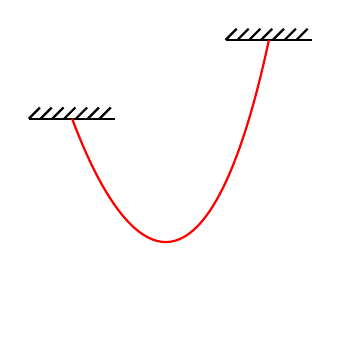
\begin{tikzpicture}[interface/.style={postaction={draw,decorate,decoration={border,angle=45,amplitude=0.2cm,segment length=1.5mm}}}]
  \draw[interface,thick] (0.2,2) -- ++(1.1,0);
  \draw[interface,thick] (2.7,3) -- ++(1.1,0);
  \draw[thick,red] (0.75,2) .. controls (1.5,0) and (2.5,-0.5)..  (3.25,3);
\end{tikzpicture}
}

\task{Маленькая шайба находится на дне цилиндрического сосуда, 
стенки которого плавно переходят в дно, образуя закругления 
пренебрежимо малого радиуса. Сосуд имеет высоту $h$ и радиус 
основания $R$. Шайба в начальный момент времени находится на 
расстоянии $L$ от центра и ее скорость перпендикулярна диаметру, 
проходящему через точку, в которой она находится. С какой 
скоростью должна двигаться шайба, чтобы вернуться в ту же точку, 
совершив $M$ оборотов вокруг центра и заехав $N$ раз на стенку? 
Напряженность поля тяжести Земли в месте, где располагается 
сосуд, равна $g$. Дно сосуда располагается горизонтально. 
Размерами шайбы и трением шайбы о дно и стенки сосуда пренебречь.}

\task{На закате человек, стоящий у озера,  видит в абсолютно 
спокойной воде отражение солнца. С какой скоростью движется это 
отражение, если в начальный момент человек видит его под углом 
$\alpha$ к горизонтали? Считать, что глаза человека находятся на 
высоте $h$ над поверхностью, а солнце садится перпендикулярно к 
линии горизонта.}

\task{Тонкий обруч, имеющий массу $М$, которая сосредоточена в оси, 
на которую он насажен, и радиус $R$, поставлен на горизонтальную 
плоскость. По гладкому каналу внутри обруча соскальзывает из 
верхней точки без начальной скорости шайба массой $m$. Определить 
скорость центра обруча, когда шайба находится в точке А (под 
углом $\varphi$ от вертикали). Трения нет.}

\task{Мальчик сидит на расстоянии $R$ от центра диска, равномерно 
раскручивающегося из состояния покоя до угловой скорости $\omega$ 
за время $T$. Какое число оборотов сделает мальчик, прежде, чем он 
начнет скользить относительно диска, если коэффициент трения 
мальчика о его поверхность равен $\mu$?}

\task{Самолет летит по прямой в горизонтальном направлении со 
скоростью $v = 720\mbox{ км/ч}$. Определите, на какую величину надо 
изменить скорость самолета, чтобы он смог описать в 
горизонтальной плоскости окружность радиуса $R = 8\mbox{ км}$. Каков 
при этом угол наклона самолета? Подъемная сила направлена 
перпендикулярно плоскости крыльев и пропорциональна квадрату 
скорости самолета (коэффициент пропорциональности в обоих 
случаях считать одинаковым) Ускорение свободного падения 
положить равным 10~м/с$^2$.}

\taskpic{Два тела связаны невесомой нерастяжимой нитью, перекинутой 
через блок, укрепленный в верхней точке наклонной плоскости с 
углом наклона $\alpha$. Получить аналитические выражения и 
построить графики зависимости силы натяжения нити, ускорения и 
силы трения в зависимости от величины массы $M$. Массу груза $m$, 
лежащего на наклонной плоскости, и коэффициент трения его о 
наклонную плоскость $\mu < \mbox{tg} \alpha$ считать известными. Трением в 
блоке и массой блока пренебречь.}{
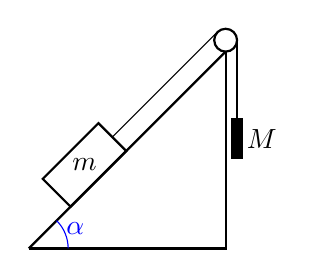
\begin{tikzpicture}
  \draw[thick] (0.5,0.5) -- (3,3);
  \draw[thick,rotate around={45:(0.5,0.5)}] (1.25,0.5) rectangle
  ++(1,0.5) node [midway] {$m$};
  \draw[rotate around={45:(0.5,0.5)}] (2.25,0.75) -- ++(1.9,0);
  \draw[thick] (3,3.145) circle (0.145);
  \draw[thick] (3,3) -- (3,0.5) -- (0.5,0.5);
  \draw (3.145,3.145) -- ++(0,-1);
  \draw[fill=black] (3+0.145/2,2.145) rectangle ++(0.145,-0.5)
  node[midway,right] {$M$};
  \draw[blue] (1,0.5) arc (0:45:0.5) node[below=3,right] {$\alpha$};
\end{tikzpicture}
}

\taskpic{Вагон длиной $4L$ и шириной $L$, стоящий на абсолютно гладких 
рельсах, заполнен водой до высоты $L$. В нем со дна всплывает 
легкий куб с ребром $L$. На какое расстояние и в какую сторону от 
точки А сдвинется вагон после успокоения воды, если плотность 
вещества куба в два раза меньше плотности воды, а масса пустого 
вагона равна массе налитой в него воды?}{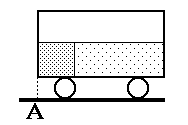
\includegraphics[width=3cm]{d10_22.png}}

\taskpic{Два стальных шарика брошены одновременно из одной точки 
горизонтальной плоскости с одинаковыми начальными скоростями в 
одном и том же направлении. Начальная скорость первого шарика 
составляет угол $\alpha_1 = 30^\circ$ с горизонтом, скорость второго --- 
некоторый угол $\alpha_2$, где $45^\circ < \alpha_2  < 90^\circ$. При полете первого 
шарика его горизонтальная координата $x_1$ изменяется по закону, 
представленному на графике. Спустя время $t  = 1{,}4\mbox{ с}$ после 
броска оба шарика оказались на одной высоте над плоскостью. 
Определите угол $\alpha_2$, под которым брошен второй шарик, а также 
расстояние между шариками через 1~с после броска. Сопротивлением 
воздуха пренебречь. Ускорение свободного падения положить 
равным 10~м/с$^2$.}{
\begin{tikzpicture}[>=latex]
   \draw[help lines,step=0.5] (0.2,-0.5) grid (3.8,4);
   \draw[thick,->] (0.5,0.5) -- (3.8,0.5) node [above left] {\tiny{$t$, с}};
   \draw[thick,->] (0.5,0.5) -- (0.5,4) node [below right]
   {\tiny{$x_1/\sqrt{3}$, м}};
   \draw[red,very thick] (0.5,0.5) -- (3.2,3.2);
   \draw (1.5,0.6) -- (1.5,0.4) node[below] {\footnotesize{1}};
   \draw (2.5,0.6) -- (2.5,0.4) node[below] {\footnotesize{2}};
   \draw (3.5,0.6) -- (3.5,0.4) node[below] {\footnotesize{3}};

   \draw (0.45,1.5) -- (0.6,1.5) node[left] {\footnotesize{5}};
   \draw (0.45,2.5) -- (0.6,2.5) node[left] {\footnotesize{10}};
\end{tikzpicture}
}

\task{Лабораторная плитка, сопротивление которой $R = 20\mbox{ Ом}$, 
включена в сеть последовательно с сопротивлением $R_0 = 10\mbox{ Ом}$. 
При длительной работе она нагрелась от комнатной температуры $t_0 
= 20^\circ\mbox{C}$ до $t_1 = 52^\circ\mbox{C}$. До какой температуры нагреется 
плитка, если ей включить параллельно еще одну такую же плитку?}

\task{Правый конец металлического стержня длиной 1~м погружен в 
ацетон, левый погружают в кипящую воду. На расстоянии 47~см от 
левого конца стержня лежит маленький кристалл нафталина. 
Сколько ацетона выкипит, пока расплавится весь нафталин? 
Считайте, что вся теплопередача происходит только через 
стержень, а поток тепловой энергии через тонкий слой прямо 
пропорционален разности температур на торцах слоя. Количество 
кипящей воды в сосуде очень велико, кипение поддерживается. 
Температура кипения ацетона $56{,}2^\circ\mbox{С}$, температура плавления 
нафталина $80{,}3^\circ\mbox{С}$.}

\task{Груженый вагон массой $M$, имеющий скорость $v$, сталкивается с 
двумя пустыми неподвижно стоящими одинаковыми вагонами, 
соединенными пружиной жесткости $k$. Чему равно расстояние между 
груженым и ближайшим к нему пустым вагоном через время $t$ после 
столкновения, если длина нерастянутой пружины равна $L$? Масса 
пустого вагона в два раза меньше массы груженного, удар считать 
кратковременным и абсолютно упругим, трением и массой пружины 
пренебречь.}

\task{На гладком горизонтальном столе покоится шар массой $m$. С ним 
упруго сталкивается клин массой $M = m/2$, движущийся углом вперед 
со скоростью $v = 5\mbox{ м/с}$. Определить, через какое время шар опять 
столкнется с клином. Угол клина $\alpha = 30^\circ$. Клин не подпрыгивает. 
Считать, что потери энергии на тепло нет.}

\task{Как опустить с крыши высотой $H = 16\mbox{ м}$ груз массой $m = 45\mbox{ 
кг}$ с помощью веревки, у которой сопротивление на разрыв равно 
400~Н? Скорость тела в момент удара о землю не должна превышать 
значения $v = 7\mbox{ м/с}$. Длина веревки немного превосходит высоту 
дома.}

\task{Длинный брусок с квадратным торцом опущен в воду, так, что 
одна из его боковых граней находится над поверхностью воды и 
параллельна ей. В таком положении брусок свободно плавает. При 
какой плотности материала бруска это возможно?}

\task{Маленький деревянный шарик с помощью нерастяжимой нити 
длиной $l = 30\mbox{ см}$ прикреплен ко дну цилиндрического сосуда с 
водой. Расстояние от центра до точки закрепления нити $r = 20\mbox{ 
см}$. Сосуд раскручивают относительно вертикальной оси, 
проходящей через центр дна. Определить угловую скорость сосуда, 
при которой нить отклоняется от вертикали на угол $\alpha = 30^\circ$.}

\taskpic{По двум кольцевым дорогам радиуса $R$, лежащим в одной 
плоскости, движутся автомобили A$_1$ и А$_2$ со скоростями $v_1 =v = 20\mbox{ 
км/ч}$ и $v_2 = 2v$. В некоторый момент автомобили находились в точках M 
и С на расстоянии $R/2$ друг от друга.
\begin{enumerate}
\item Найдите скорость автомобиля А$_2$ в системе отсчета, связанной 
с автомобилем А$_1$ в этот момент.
\item Найдите скорость автомобиля А$_2$ в системе отсчета, связанной 
с автомобилем А$_1$, когда А$_2$ окажется в точке D.
\end{enumerate}
Размеры автомобилей малы по сравнению с $R$.}{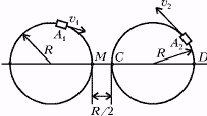
\includegraphics[width=4cm]{d10_31.png}}

\taskpic{Тонкостенная цилиндрическая трубка массы $m$ катится без 
проскальзывания по горизонтальной поверхности неподвижной 
плиты П со скоростью $v$ и попадает на ленту горизонтального 
транспортера, движущегося в том же направлении со скоростью $u$. 
Коэффициент трения скольжения между трубой и лентой равен $\mu$.
\begin{enumerate}
\item Через какое время $t$ после вкатывания на ленту трубка начнет 
катится по ней без проскальзывания?
\item Определите изменение кинетической энергии трубки за время $t$.
\item Чему равно количество теплоты, выделившееся за время $t$?
\end{enumerate}}{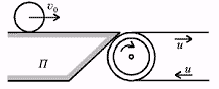
\includegraphics[width=4cm]{d10_32.png}}

\taskpic{По гладкой горизонтальной поверхности скользит палка 
длиной $2L$, вращаясь с угловой скоростью $\omega$. Ее центр движется 
прямолинейно со скоростью $v$. Далеко впереди на расстоянии $L/2$ от 
линии движения центра палки находится маленькая кегля. При каких 
значениях $\omega$ палка обязательно собьет 
кеглю?}{
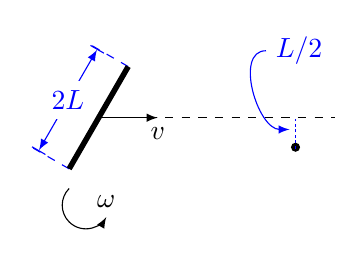
\begin{tikzpicture}[>=latex]
   \draw[dashed,blue,rotate around={60:(0.5,1.5)}] (0.5,1.5) -- +(0,0.6) node [coordinate, near end] (a) {};
   \draw[dashed,blue,rotate around={60:(0.5,1.5)}] (2,1.5) -- +(0,0.6) node [coordinate, near end] (b) {};
   \draw[blue,|<->|] (a) -- node[fill=white] {$2L$} (b);
   \draw[line width=2pt,rotate around={60:(0.5,1.5)}] (0.5,1.5) --
   ++(1.5,0);
   \draw[dashed] (0.5,1.5) ++(60:0.75) -- + (3,0);
   \draw[->] (0.5,1.5) ++(60:0.75) -- + (0.75,0) node [below] {$v$};
   \draw[->] (0.5,1.25) arc (135:330:0.3) node[above] {$\omega$};
   \filldraw[black] (0.5,1.5) ++(60:0.75) ++(2.5,0) ++(0,-1.5/4)
   circle (0.05) node (c) {};
   \draw[blue,dashed,dash pattern=on 1pt off 1pt] (c) ++(0,-0.02) -- ++(0,1.5/4);
   \draw[blue,->] (3,3) node [right] {$L/2$} to[out=180,in=180] (3.3,2);
\end{tikzpicture}
}

\taskpic{На вертикальный цилиндрический стержень радиуса $R$ 
насажено устройство, состоящее из корпуса, в котором находятся 
два груза одинаковой массы $M$, прижимаемые к стержню с помощью 
двух одинаковых пружин жесткостью $k$. Устройство вращается 
вокруг стержня с постоянной угловой скоростью $\omega$ и движется 
вниз. Найти установившуюся скорость движения устройства вниз, 
если коэффициент трения грузов о стержень равен $\mu$ и пружины 
сжаты на величину $x$. Массой всех остальных деталей пренебречь. 
Ускорение свободного падения $g$.}{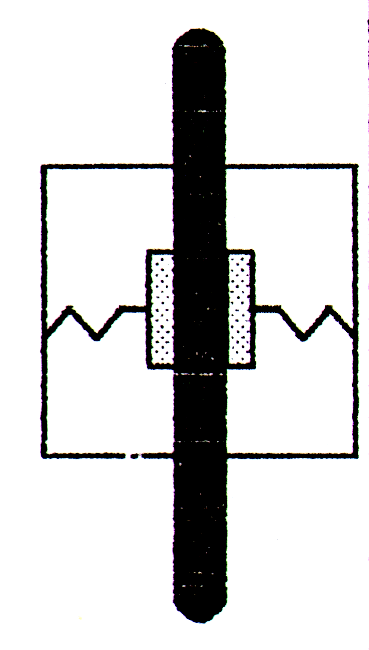
\includegraphics[width=2cm]{d10_34.png}}

\task{Птица летит горизонтально на высоте $H$ с постоянной скоростью 
$u$. Плохой мальчик замечает птицу в момент, когда она находится в 
точности над его головой, и сразу же стреляет из рогатки. Какой 
должна быть скорость птицы, чтобы мальчик не смог попасть в нее, 
если максимальная скорость вылета камня равна $v$? Сопротивлением 
воздуха пренебречь.}

\task{Внутри куба вырезана сферическая полость таким образом, что 
центр сферы находится над центром нижней грани куба. Полость 
наполовину заполнена жидкостью плотностью $\rho_2$. Куб очень 
медленно наклоняют через ребро АА. При каком угле наклона куб 
опрокинется? Длина ребра куба в $n$ раз больше радиуса полости $r$, а 
центр полости расположен на высоте $kr$ над основанием куба, 
причем $k > n/2$. Плотность вещества куба $\rho_1$. Объем шара радиуса $r$ 
равен $\frac43\pi r^3$.}

\task{Однородный стержень массой $M$ подвешен при помощи легких 
нерастяжимых нитей одинаковой длины к потолку и находится в 
положении устойчивого равновесия. По стержню без трения может 
перемещаться небольшая шайба массой  $m$. В начальный момент 
конструкцию отклоняют на угол $\alpha$ от вертикали в плоскости 
подвеса и отпускают, при этом шайба находится посередине 
стержня. Найти ускорение шайбы в начальный момент.}

\task{Доска 1 лежит на такой же доске 2. Обе они как целое скользят по 
гладкой ледяной поверхности со скоростью $v$ и сталкиваются с 
такой же доской 3, верхняя поверхность которой покрыта тонким 
слоем резины. При ударе доски 2 и 3 прочно сцепляются. Чему равна 
длина каждой доски, если известно, что доска 1 прекратила 
движение относительно досок 2 и 3 из-за трения после того, как она 
полностью переместилась с 2 на 3? Все доски твердые. Коэффициент 
трения между досками 1 и 3 равен $k$. Трением между досками 1 и 2, а 
также трением досок 2 и 3 о лед можно пренебречь.}
